\documentclass[12pt,oneline,a4paper,numbib]{ouparticle}
\usepackage{array,multirow,graphicx}
\usepackage{pdflscape}% for landscape

\usepackage{adjustbox}     % adjusting table (too wide)
\usepackage{rotating}      % sidewaytables
\usepackage{array}
\usepackage{stackengine}

\usepackage{amsmath} % \numberwithin{equation} doesn't exist without this package.
\numberwithin{equation}{subsection} % This line resets equation numbering when starting a new section.
\renewcommand{\theequation}{Eq. \thesubsection.\arabic{equation}} % This line ads "Eq." in front of your equation numbering.

\providecommand{\e}[1]{\ensuremath{\times 10^{#1}}}

\begin{document}

\title{Modelling long-term effects of management strategies in mixed fisheries}

\author{%
\name{Nekane Alzorriz}
\address{European Commission, Joint Research Centre (JRC), Sustainable Resources Directorate, Water and Marine Resources Unit, Via Enrico Fermi 2749, 21027 Ispra, Italy.}
\email{nekane.alzorriz@gmail.com}
\and
\name{Adriaan Rijnsdorp}
\address{Wageningen Marine Research, PO Box 68, 1970 AB IJmuiden, The Netherlands.}
\email{adriaan.rijnsdorp@wur.nl}
\and
\name{Jan Jaap Poos}
\address{Wageningen University, The Netherlands.}
\email{janjaap.poos@wur.nl}}
%Most worldwide fish stocks are overexploited, and so exploited beyond the maximum sustainable yield (MSY). 
\abstract{The EU common fisheries policy (CFP), designed for the long-term environmental, economic, and social sustainability of fishing and aquaculture activities, includes making use of the maximum sustainable yield (MSY) reference points as targets for exploiting commercially important fish stocks. To incentivise individual business to improve selectivity and avoid unwanted catches, it also introduced a landing obligation. Achieving these complex objectives may not necessarily reduce harvest rates, but will change the underlying selectivity patterns of harvests. The impact of exploiting at MSY and no discarding allowance on the optimal effort allocation between fleets is analyzed. We contrast two management plans to achieve MSY from two stocks and compare their effectiveness based on a management strategy evaluation that uses a dynamic state variable model including errors in decision-making in its operating model. The results show that when accounting for quota on one specie and for quotas on both species, MSY landings in the short-term are 30\% to 50\% lower than when compared to an unmanaged situation simulations. Some years after the implementation, MSY landings are similar or 25\% to 50\% higher than the pre-manage situation. Optimal effort at MSY generates effort reductions of 37\% to 62\% over the mid-term, thus there would be some vessels that could benefit up to 1.4 times larger profits than before the CFP implementation. The results show that for both species, any of the two management plans would be beneficial to both the stock and part of the fleets over the mid-term compared with the projections over the short-term.}

\date{\today}

\keywords{management strategy evaluation; dynamics state variable model; errors in decision-making; landing obligation; maximum sustainable yield, common fisheries policy}

\maketitle

\section{Introduction}
%We have to make sure we are clear on the ages of the species: do we start at 0 or at 1?

Management strategy evaluation (MSE; \cite{Bunnefeld2011, Sainsbury2000, Smith1994}) seeks to study the implications of management strategies using simulations \cite{Punt2016}. Such simulations should include all important processes of a fishery. Any fishery is inherently a socio-ecological system, with coupled dynamics of fishing fleets, exploited stocks, and their governance \cite{Punt2016, Rasemeyer2007}. Given the complexity of socio-ecological system the uncertainy about the dynamics and feedbacks are considerable. As a result, any forecasted success in achieving goals of management strategies may thus be small compared to system stochasticity, or worse, be counteracted by unintended consequences of the management strategy. The robustness of management strategies to the uncertainty in the processes that govern fisheries systems thus need to be accounted for \cite{Andersen2010, Kell2007, Prellezo2016, Punt2016}. 

The adaptive response of fishers to their environment is one of the key uncertainties requiring attention in MSE \cite{Fulton2007}. Simulation tools for such a response are available, borrowing methodology from state-dependent foraging decisions in ecological systems \cite{ClarkandMangel2000,Houston1999}. State-dependent behaviour of individual fishing vessels, aggregated into fleet dynamics, have been developed using stochastic dynamic programming \cite{Alzorriz2018,Batsleer2015, Dowling2011, Poos2010, Gillis1995}. These models generally predict short term (within a fishing trip, or a quota year) effects of changes in management or the environment by determining which choices yields the best chance of increasing utility, while keeping track of the state of each individual. The effect of a choice on utility depends on the state of the individual, the economic environment, such as fuel prices, and the biological environment, such as the spatial distribution of resources. 

Using dynamic variable state models, effects of e.g. relocation costs of marine protected areas have been modelled \cite{Dowling2011}. Dynamic state variables have also been used to describe discarding behaviour \cite{Batsleer2015, Batsleer2013, Gillis1995, Alzorriz2018}. Some of these studies have tried to shed light on the potential outcomes of the European fisheries management reform of 2013. That reform included using the use of the maximum sustainable yield (MSY) reference points as targets for exploiting commercially important fish stocks and the gradual introduction of a landings obligation (LO) \cite{CFP2013}. Indeed, using spatial and temporal distributions of catch rates within a single year, dynamic state variable models forecasted high costs in mixed fisheries in the short term as a result of the LO \cite{Alzorriz2018, Batsleer2013, Batsleer2015}. These costs result from removing the choice to discard part of the catch and in doing so adapt landings to quota \cite{Alzorriz2018}. This will result in fishing effort reallocation and early closures of fisheries once quota have been reached. 

Meanwhile, the LO potentially improves selectivity of fisheries by providing incentives to move away from areas with high levels of unwanted catch and the use of more selective gears \cite{Alzorriz2016, Alzorriz2018}. The improved selectivity should lead to higher long term catches. These long term benefits to fisheries that could result from improved selectivity under the LO are ignored in previous studies on the adaptive response of fisheries \cite{Batsleer2015, Batsleer2013, Alzorriz2018}. Ignoring the potential for improved selectivity leaves out a key element in the perceived benefit of the LO. In mixed fisheries, however, optimizing single species selectivity and achieving MSY while landing all commercial catches is challenging because of trade-offs in the catches of different species and size-classes \cite{Batsleer2013, Ulrich2017}. Forecasting whether any management will be effective requires understanding the response of fishers constrained by these trade-offs and the effects of the response on the development of fish populations \cite{Venables2009}. If the fleet dynamic model results in a short term movement of vessels to allocate effort both spatially and temporally, we also expect longer term changes to occur in fish populations and the economy of the fishery \cite{Alzorriz2018}.

We present an MSE framework that couples forecasts from a state-dependent behaviour model to a biological dynamic models that forecasts population effects resulting from the collective fishers behaviour. The model includes the (real or perceived) local biomass of two populations, governed by growth, mortality, and migration. These populations are size-structured, and are modelled in a spatially heterogeneous environment. The populations are harvested by a single fleet that has annual fishing rights for both populations, consisting of individuals who make monthly choices on fishing locations. These choices depend on the perceived spatial distributions of biomasses, but also on various costs, principally that of fuel. The constraints on the fleet  includes management-imposed constraints such as fish quotas. In the framework, these quotas are decided by a a management body that observes the total biomass of the two stocks and with the goal of constraining fishing mortality so that maximum sustainable yields are achieved.   

The MSE framework is used to understand the fleet dynamics in a spatially and temporally heterogeneous mixed quota-regulated fishery when reducing from unmanaged (unconstrained catch quota) to MSY managed combined with the LO where discards are not allowed, and to compare it in order to assess on the biological and economic consequences. If LO and catch quotas are not fully enforced, there will be an incentive to continue discarding. Therefore, this manuscript tends to understand the likely adaptive change in fishing patterns that will help us to understand if this leads to a better balance between quotas and catches.

\section{Methods}

The management strategy evaluation framework was used to forecast the dynamics of a hypothetical mixed fishery on two species. In the fishery, there are three essential elements: (i) a collection of size structured fish stocks, whose dynamics are governed by annual reproduction, growth, migration, and mortality; (ii) a management body that evaluates the fishing pressure and aims to set annual quotas in accordance with fishing mortalities dictated by $H_{max}$ reference points (harvest at maximum sustainable yield); and (iii) a fleet of individual fishers who aim to make the best use of their annual quota. Within this mixed fishery, individual vessels make adaptive choices about fishing location and discarding that depend on the distribution of the resources, and the quota that hold. Each of these elements is discussed in more detail below. The essential elements of the framework are summarized in Figure \ref{fig:MSE} and \ref{fig:stockdyn}.

The framework consists of an operating model (OM) and a management procedure (MP). The OM captured the key processes in the dynamics of the fish populations, the fisheries, and the management body, and can be thought of as a minimum realistic model \cite{Punt1995}. The OM thus includes individual harvester decision-making (including error) and the consequent biomass of fish stocks, including the essential elements for calculating the individual harvester economic performance (Fig. \ref{fig:stockdyn}). The management body used the MP to make its decision on how to respond to the state of the resource. This MP thus includes the data collection from the fishery, how these are interpreted, and the harvest control rule (HCR) that dictates the limits that are set to the fishery. 

 
\begin{figure}[!h]
\centering
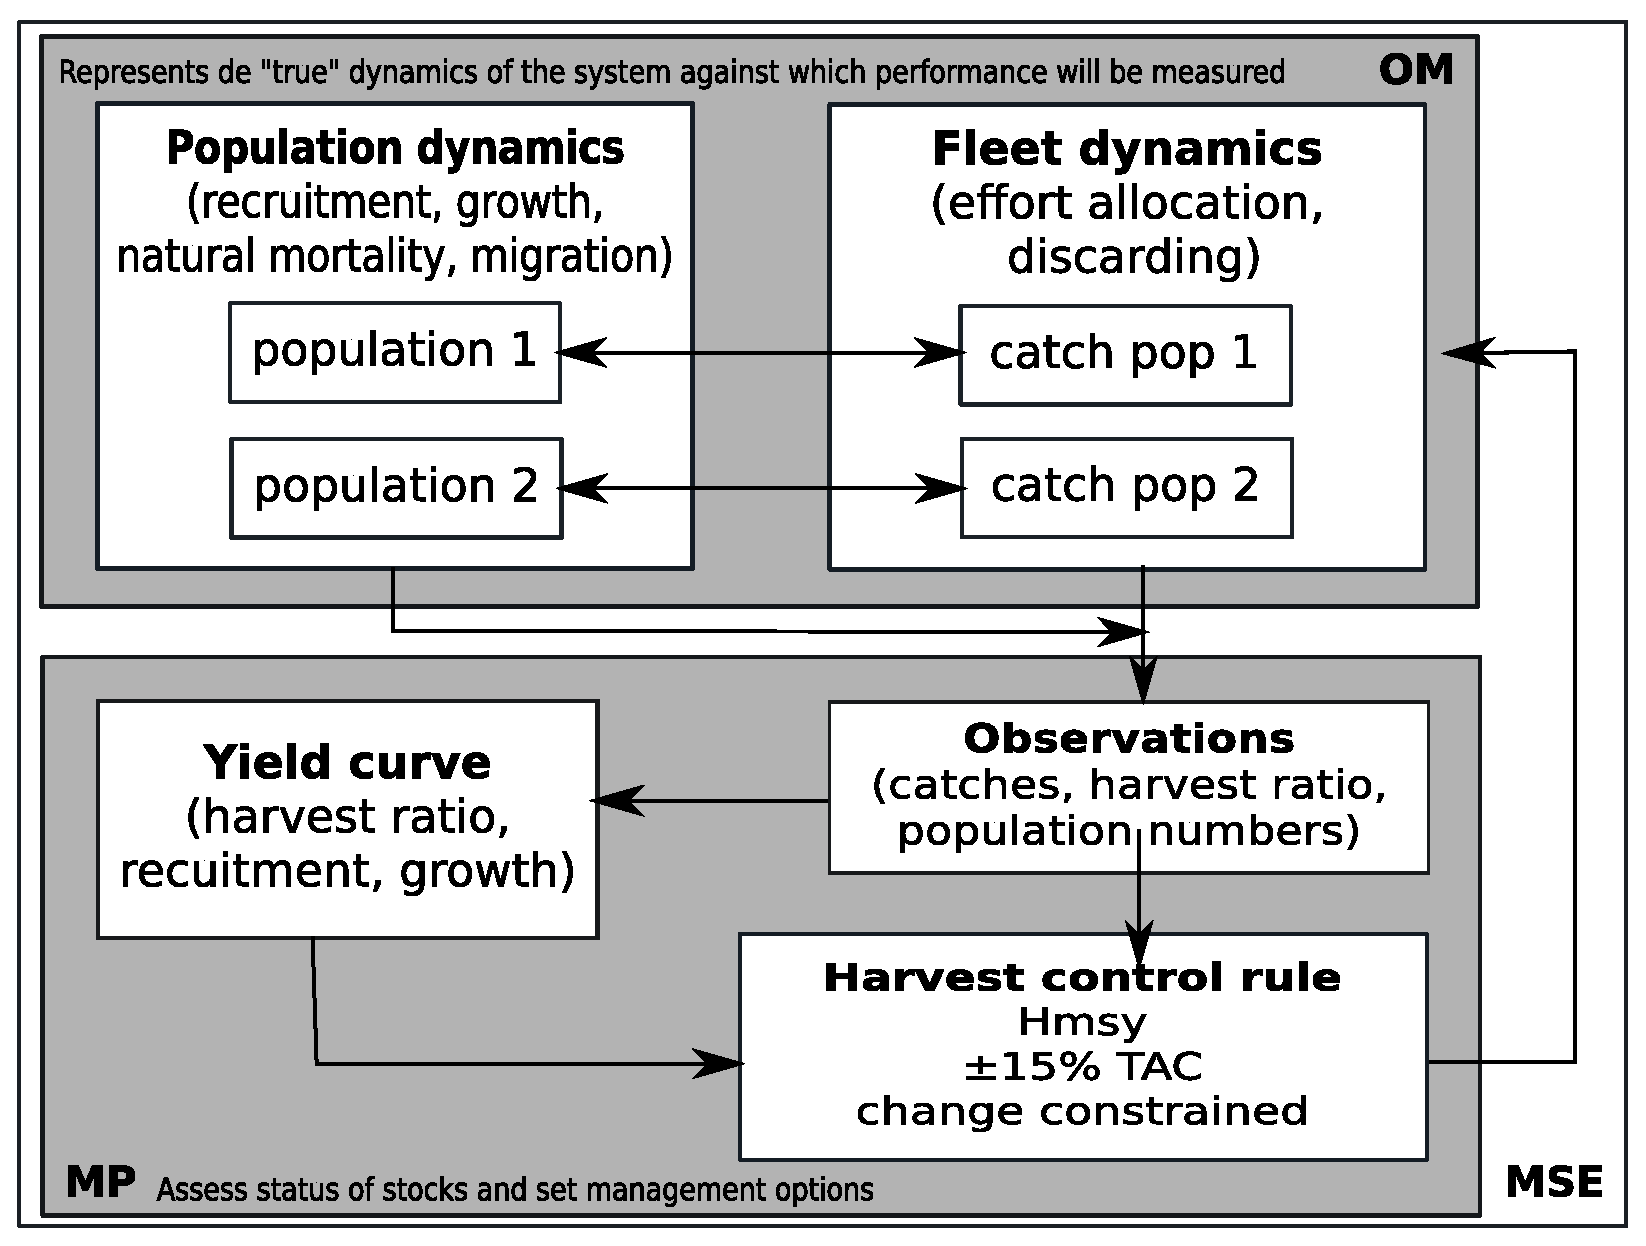
\includegraphics[width=0.55\textwidth]{Figures/MSE.eps} 
\caption{Conceptual overview of the MSE approach, including the OM and the MP components of the framework.}
\label{fig:MSE}
\end{figure}

\begin{figure}[!h]
\centering
\includegraphics[width=0.4\textwidth]{Figures/Areadynamics.eps} 
\caption{The OM component, including the key processes in the dynamics of the fish populations.}
\label{fig:stockdyn}
\end{figure}

\subsection{Population dynamics}


To allow the fishery to make spatial and temporal choices, the model needed to be seasonally and spatially explicit. The dynamics of the fish stocks were modelled using an age-structured model that was spatially explicit, with seasonal time steps. In each seasonal time step, fish grow, migrate, and die. The number of fish of stock $i$ of age $a$ at year $y$, in season $s$, and area $p$ was written as $N_i (a, y, s, p)$. The ages in the model range between age 0 and age $A$, the maximum age in the model. The seasons range between season 1 and season $S$, the last season within each year. Individuals were born at age 0, at the start of each year $y$, in season 1. The number of recruits $R_i (p)$ in the model was a function of the area $p$ and independent of the size of the adult population. The population numbers at age 0 are thus
 
\begin{equation}
N_i (0, y, 1, p) = R_i (p).
\end{equation}

Mortality in the model resulted from fishery catches and natural causes such as predation, diseases, and senescence. The decrease in population numbers was thus the result of the catches ($C_i (a, y, s, p)$) and a natural mortality constant $M_i$ that described natural mortality as a fixed fraction of the population. These mortalities reduced the population numbers among a cohort of fish. Because the model was seasonally structured, the population numbers for seasons 2 to $S$ were dependent on the previous season,

\begin{equation}
N_i (a, y, s+1, p) = N_i (a, y, s, p) - C_i (a, y, s, p) - M_i N_i (a, y, s, p) . 
\end{equation}

Likewise, the population numbers in season 1 depended on the numbers in season $S$ of the previous year,

\begin{equation}
N_i (a+1, y, 1, p) = N_i (a, y, S, p) - C_i (a, y, S, p) - M_i N_i (a, y, s, p). 
\end{equation}

Migration for each species was defined by an array $D_i (a, s, em, im)$ that defined immigration and emigration on a given stock relative to the stock sizes. The size of that array was defined by the number of age classes, seasons and number of areas. emigrants leave area $em$ and move to area $im$. The emigrated part of the population is then subtracted from each of the areas, so that that population numbers per year and season remain unaffected by migration.

Individual body growth was modelled by a von Bertalanffy growth equation to convert numbers to lengths, and an allometric equation to convert length to weight. The weights for individuals in the stock and in the catches are thus calculated as

\begin{equation}
w_i(a,s) = \alpha * ( L_{\infty_i} * (1-\exp^{(-K * (a+(s/S)))}))^{\beta}.
\end{equation}

The realized catches are the sum of all individual catches resulting from the dynamic state variable model. The model inputs consist of the expected individual catch rates, which are random variables. These random variables were normally distributed, with means $\hat c_i (a, y, s, p)$ being a function of population size, age dependent catchability $q_i (a)$ in any year, season, and area,

\begin{equation}
\hat c_i (a, y, s, p) = N_i (a, y, s, p) * q_i (a) * w_i(a,s).
\end{equation}
The standard deviations $\Sigma_i (a, y, s, p)$ of the catch distributions were constant fraction their means, using a ratio $\eta$. 

\subsection{Fleet dynamics}

A dynamic state variable model was used to simulate a fleet of individual fishing vessels \cite{Alzorriz2018, Batsleer2015, ClarkandMangel2000, Dowling2011, Houston1999, Poos2010}. The model structure was equal to \cite{Alzorriz2018}. Each individual vessels had a set of choices, which include the choice to go fishing in a season, location choice within that season. No discarding was allowed in the model. The model had annual fines for exceeding landings quota as in \cite{Alzorriz2018}. In order to calculate state dependent choices during the year, we started by defining the annual fines for exceeding landings quotas at the end of the year:
\begin{equation}
\Phi (C_i, Q_i, F_i)= -\sum_i (\textrm{max}( 0, (C_i - Q_i))* F_i),
\end{equation}

where $C_i$ was the cumulative annual catches for species $i$ for an individual vessel. These cumulative catches defined the state of the individual. $Q_i$ was the annual individual quota for catches for the different species. Individual quotas were not transferable. $F_i$ was the fine per unit weight for exceeding individual catches quota.

The maximum expected utility between current season $s$ and the end of the year was $V (C_i, Q_i, F_i, s)$, and the model started by setting $V (C_i, Q_i, F_i, S)= \Phi (C_i, Q_i, F_i)$. For preceding seasons, the expected utility depended on individual choices, and each time step individuals chose to visit fishing area $p$, or to stay in port. While fishing, any combination of the age classes caught of the quota species had to be landed. The expected utility for each state and each time step $s$ was calculated backward using stochastic dynamic programming \cite{ClarkandMangel2000}:
\begin{equation}
V (C_i, Q_i, F_i, s) = max_{p}( R(p, s)- G(p) - C(p) + E_{p}[V (C_i^\prime, Q_i, F_i, s+1)]),
\end{equation}

where $R(p, s)$ was the expected immediate contribution of the gross revenue from the sales of fish in a season resulting from choices $p$ (gross revenues resulted from multiplying catches different age classes of species 1, species 2 and prices). Prices of fish were assumed to be dependent over fish age (subsection size dependent pricing). $G(p)$ represented the incurred fuel costs per season from the choice of fishing area $p$, while $C(p)$ represented the variable operating costs (crew share, gear maintenance and landing costs, Table~\ref{t:fishery}), which in turn depended on the change in cumulative catches and fish prices. The term $E_{p}[V (C_i^\prime, Q_i, F_i, s+1]$ denoted the expected future utility taken over all possible states resulting from choices $p$. The transition of these states were based on normal distributions of catch rates, using the means and variances for the species, as explained in the model conditioning section, following \cite{Poos2010}.

Rather than assuming that each individual always made the optimal choice, we assigned a probability to each choice proportional to its expected utility, following \cite{Dowling2011}. The expected utility for any choice was
\begin{equation}
U (C_i, Q_i, F_i, s) = R(p, s)- G(p) - C(p) + E_{p}[V (C_i^\prime, Q_i, F_i, s+1)].
\end{equation}

If $U^*$ was the expected utility at the optimal choice for a given t, we set

\begin{equation}
\Delta_{p}(C_i, Q_i, F_i, s) = U^* (C_i, Q_i, F_i, s) - U (C_i, Q_i, F_i, s),
\end{equation}

and then defined the probability of a choice for a given area and discarding as	

\begin{equation} \label{eq:solve}
P_{p}(C_i, Q_i, F_i, s) = \frac
                % Nominator
                {e^{ -\Delta_{p}(C_i, Q_i, F_i, s)/\sigma}}
                % Denominator
                {\sum_p e^{ -\Delta_{p}(C_i, Q_i, F_i, s)/\sigma}},
\end{equation}
where $\sigma$ was a tuning parameter that measured how important it was to be near the optimal choice. A large $\sigma$ resulted in uniform probabilities of choices, with vessels being distributed uniformly across the different fishing areas. In contrast, a small $\sigma$ forces vessels to concentrate in the optimal location (but note that $\sigma$ should be $> 0$). For computations, we used $\sigma = 65000$ (Table \ref{t:fishery}). %(noting that $\Delta$ ranged from 0 to $\sim 2 x 10^{3}$, but was generally of the order of $1 x 10^2$ in magnitude).

The dynamic state variable model was solved for each year by iterating backwards in time, while finding the probability distribution choice in terms of location for all possible states, combining the net revenue obtained from the sale of fish and costs of a fishing trip and the effect of the annual fines when exceeding annual quota. Further details for this procedure can be found in \cite{Alzorriz2018, Batsleer2016} and \cite{Dowling2011}.

Once the backward calculations were finished, the forward part is a Monte Carlo simulation where the probabilities of choices were sampled randomly using the probabilities in~\ref{eq:solve}. For each year, these forward Monte Carlo simulations determine the fishing effort in each season and area $E(y,s,p)$, and the catches $C_i (a, y, s, p)$ for each age in each season and area. The effort allocation component of the operating model provides the link between the management decisions and the biological component of the operating model.


\begin{table}[!h]
\centering
\caption{Model parameters.}
\label{t:fishery}
\resizebox{0.6\textwidth}{!}{%
\begin{tabular}{@{}llr@{}} 
\hline

\textbf{Population dynamics}                                    &                \\ \hline
&  \\%& & \\

number of recruits                                          & $R_i (p)$           & 500               \\
maximum age                                                 & $A$                 & 6               \\
number of areas                                             & $p$                 & 2               \\
number of months                                            & $S$                 & 12               \\
natural mortality                                           & $M_i$               & 1\e{-4} \\ %0.0001     \\
Asymptotic length                                           & $L_{\infty_i}$      & 50            \\
Growth rate                                                 & $K_i$               & 0.6         \\
Length-weight conversion factor                             & $ \alpha_i$         & 2\e{-4} \\% 0.0002   \\
Length-weight isomorphy factor                              & $\beta_i $          &   3              \\
Migration                                                   & $D_i $              & 2.5\e{-2} \\%  2.5\%              \\
&               \\
\textbf{Fleet dynamics}                                     &               \\ \hline   
&  \\%& & \\

Number of vessels                                           &                       & 8000           \\ 
Fuel costs (Euro fishing month\textsuperscript{-1})         &                       & 2000        \\ 
Gear maintenance (Euro fishing season\textsuperscript{-1})  &                       & 0               \\ 
Crew share                                                  &                       & 0\%        \\ 
Landing costs (Euro t\textsuperscript{-1})                  &                       & 0               \\
Optimal choice error                                        & $\sigma $             & 65000            \\ 

&                 \\  
\textbf{Fishery }                                           &             \\ \hline   
&  \\%& & \\

Intial quota  (kg vessel\textsuperscript{-1})               &                       & 200 \\%& & \\
catchability                                                & $q_i (a)$             & 2.5\e{-5} \\%0.000025        \\ 
effort (p,s)                                                &                       & 1                 \\ 
Price of species at mean weight (Euro kg\textsuperscript{-1})& $\bar{p}_i$          & 30             \\
Slope of species price                                      & $\gamma_i$            & 15            \\
Fine for overshooting quota  (Euro kg\textsuperscript{-1})  &  $F_i$                & 3000              \\
Ratio of standard deviations to catch means                 & $\eta$                & 0.08           \\ 
&                 \\  \hline%& & \\\hline
\end{tabular}
}
\end{table}

\subsubsection{Size dependent pricing}

Prices of fish were assumed to be fixed over time but influenced by the body weight of the individuals in the catch, as is commonly observed \cite{Zimmermann2011, Zimmermann2013}. Following \cite{Zimmermann2011}, the relationship between fish price and body weight was modelled as:
\begin{equation}
 p_i (a,s) = \bar{p}_i + \gamma_i \times \frac{w_i (a,s) -\bar{w_i}}{\bar{w_i}},
\end{equation}
where $p_i (a,s) $ is the price of species $i$ at age $a$ and season $s$. The price was a linear function of the weight of individuals of species $i$ at age $a$ and season $s$. $\bar{p}_i$ is the price of the species at the mean weight over the age range. The mean weight over the age range is $\bar{w_i}$. $\gamma_i$ gave the price increase when individual mass was increased by $\bar{w_i}$. 

\subsection{Case study parametrization}

To mimic spatially heterogeneous fish populations in a mixed fishery where fishers make sequential choices on fishing areas, the model was divided into a 'north' and 'south' area, and twelve fishing seasons per year (Table \ref{t:fishery} and Fig. \ref{f:distribution}). There were two fish species in the model, both of which are caught by the fishery. The annual number of recruits was equal for the two species, and arbitrarily set to 500 per year (Table \ref{t:fishery}). The species differed with respect to their nursery grounds: all individuals of species 1 were born in the northern area, while all individuals of species 2 were born in the southern area (Fig. \ref{f:distribution}). The maximum age that any individual can reach was 6 years old. During their life, individuals grew in length towards the asymptotic length, which was 50 cm for both species (Table \ref{t:fishery}). Conversion from length to weight was also equal for the two species (Fig. \ref{f:prices}). Migration was parameterized so that a gradual diffusion occurred between the two areas, equal to 2.5 percent of the difference in abundance (Table \ref{t:fishery}). For the unfished situation this led to a clear segregation of the younger ages over the two areas, while the older ages were equally distributed over the two areas (Fig. \ref{f:distribution}). Mortality from natural causes such as predation, diseases, and senescence was assumed to be negligible, and $M_i$ set to 0.0001. Although such absence of natural mortality impossible in reality, one could argue that the model thus mimicked long-lived species.

\begin{figure}[!ht]
\centering
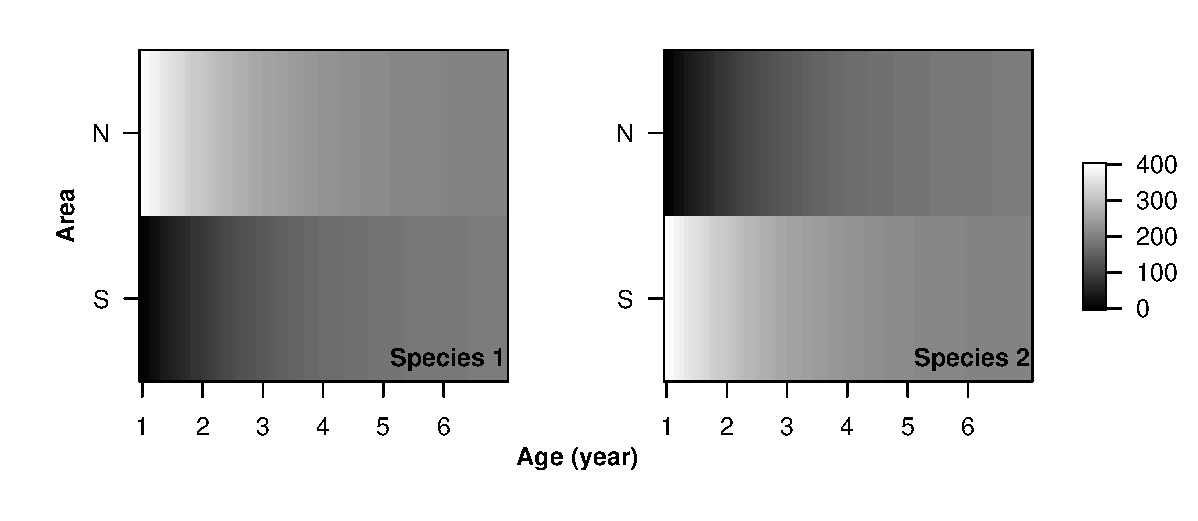
\includegraphics[width=0.8\textwidth]{Figures/Distributions.eps} 
\caption{Biomass distribution in numbers over the areas as a function of age when stocks are in virgin stock status for species 1 (a) and species 2 (b). For species 1 nursery ground occurs in the northern area, while species 2 in the southern area (high biomass in white). Over the two areas, initial biomass distribution shows a clear segregation of the younger ages (high and low fish biomass, in white and black respectively), while the older ages show similar distributions (grey colours).}
\label{f:distribution}
\end{figure}

Age-dependent catchability linked the population biomasses to the catches in the fishery, and was thus one of the crucial parameters determining the interaction between the two. In the case study, this age-dependent catchability $q_i (a)$ was assumed independent of age $a$, and equal for the two species (Table \ref{t:fishery}).

The mean prices for the two species were set to 30 euro per kg, ranging between 17.3 euro per kg for the youngest age and 36.5 euro per kg for the oldest age (Table \ref{t:fishery} and Fig. \ref{f:prices}). The fines for overshooting the quota was set to 3,000 euro per kg (Table \ref{t:fishery}). These high fines combined with an assumed 100\% detection of exceeding quotas resulted in model results in which fishers comply with quota regulations.

\begin{figure}[!ht]
\centering
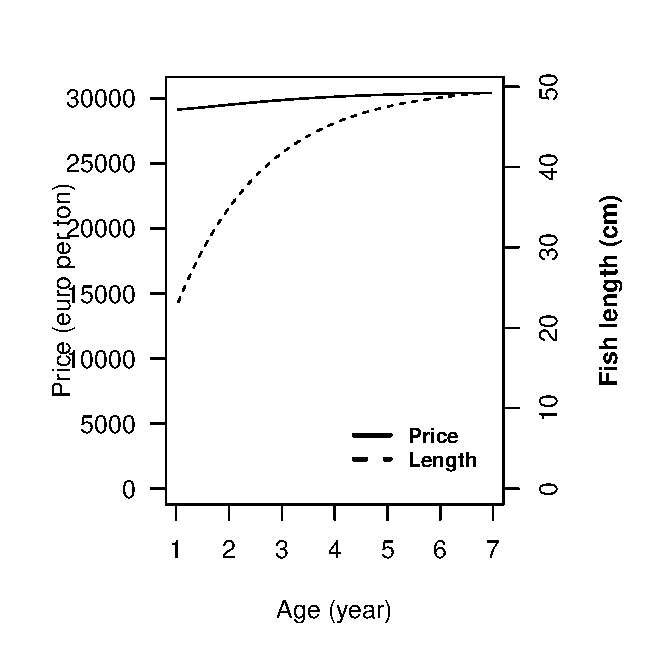
\includegraphics[width=.5\textwidth]{Figures/Prices.eps} 
\caption{Lengths and prices of the two species.}
\label{f:prices}
\end{figure}

\subsection{Management procedure}

The management model encompassed the harvest control rules. The HCRs referenced to biological reference points ($H_{max}$) to produce management actions in the form of a harvest or effort level: changes in selectivity or spatial and temporal reallocations or restrictions of fishing effort. The input to the fisheries model consisted of the expected catch rates and the individual quota that were set for each individual in the fleet. These individual quota were set in a management procedure, which mimicked the decisions of a management body. This management body made observations on the state of the resources, and the exploitation characteristics of the fishery. In the model, the management body was assumed to collect annual observations of the biomass of the stocks, including the distribution of the biomass over the different ages. These observations stem from fisheries independent observations, such as surveys with known catchabilities. In addition, the management body made annual observations of the catches, including their age distribution. 

The observed biomass and catches allowed for estimation of the annual harvest rates ($H_i$), and the estimation of a yield per recruit curve, that was dependent on fish growth and mortality. The yield curve was dome shaped, with a maximum that is called $H_{i,max}$. Fishing at a harvest rate that is equal to $H_{i,max}$ should lead to maximum sustainable yields. The yield per recruit curve omitted the potential effect of the feedback between adult biomass and recruitment, which anyway was absent in the population dynamics, that assumed a constant recruitment. The HCR used by the management body resulted in annual quotas such that the harvest rate in a year corresponded to $H_{i,max}$. These quotas were then divided equally over the individual vessels in the simulations.

\begin{equation}
 Q_{i,y+1} = \frac
                % Nominator
                {\sum( [\frac{H_{i,max}(a,y,s)}{\bar{H_i(a,s)}} \times H_i(a,s) \times sum( N_i (a, y, s, p))] \times w_i(a,s)) }
                % Denominator
                {number\  of\  vessels}.
\end{equation}


\subsection{Scenarios}

The model was set up in three consecutive time windows. The first window of 10 years was enough to get to stable populations. During this first period, new young individuals entered the population in the absence of fishing. This resulted in a virgin stock status. The consecutive 15 years, the fleet of 8000 vessels started fishing in the absence of any fisheries regulations. During this time window, the fishery was unmanaged, with unlimited quota for both species (pre-manage period). During the last 15 years of projections, the management procedure was introduced, the fishery was constrained by setting MSY targets while discarding was not allowed (post-manage period). 

Two management scenarios were examined in the model. The two scenarios differ in the number of stocks under quota. In the "single-species catch quota" scenario quota on species 1 was controlled by the HCR. In the "both-species catch quota"  quotas on both species were controlled by HCRs. The comparison among these scenarios allowed the evaluation of costs and benefits, both economic and in terms of risks to both stock and livelihoods, that resulted from the response of individual effort allocation to meet the objectives of the landing obligation regarding the objectives of the CFP, specially the MSY. To be able to analyse the results of this complex actions of implementing the MSY and the LO, we simulated the effects of implementing the LO without any exceptions or flexibility. When necessary, for example, in the case of estimating the modelled monthly mean of harvest rates, 5 years windows were selected to characterise the fleet in that pre- and post-manage period for both species (grey and green areas in Fig. \ref{f:catches}, respectively).
 

%changes in selectivity.
%These management scenarios were chosen such that, if the management model was the correct model of reality, the corresponding equilibrium state of the system would meet the objective of the plan. 

\section{Results}

% CATCHES
Stochastic simulations were carried out for the management scenarios contemplated: moving from an unmanaged period to a situation where one or both species were regulated by quotas and forced to keep fishing mortality below the MSY, while it was not possible to discard. 

Figure \ref{f:catches} shows the expected catch of the two target species and the impact of implementing the management scenarios on simulated catch. When the fishery was unmanaged, the observed harvesting rates showed average values larger than the estimated average values that can be harvested in a sustainable manner ($H_{max}$), thus resulted in a situation where the stocks were overfished, reaching total catches of more than 4 tons per species. In both scenarios, the introduction of PM caused an immediate reduction in catches of target species in the short-term. However, after such a reduction in the initial years, the stock biomass increases in the mid-term (after a transition of $<$5 years), and therefore mid-term TACs and catches were higher than before the implementation of the MP (Fig. \ref{f:catches}, c and d). The most notable differences in catch between the different scenarios lied in the absence of a regulatory quota for species 2. In the case where the fishery was limited only by HCR for species 1; higher catches for species 1 were observed in the mid-term. While species 2 maintained similar catches to those observed in the absence of management. As there was no quota restriction on species 2, catches of species 1 were adjusted to the estimated TAC in the HCR (Fig. \ref{f:catches}, a and b). However, for the fishery that was governed by quotas on both species, differences between catches and quotas were more noticeable due to the choke effect. As there was a similar spatial overlap of mature species and an antagonic spatial distribution of young species between the two fishing areas (Fig. \ref{f:distribution}), some fishing opportunities would always be lost for keeping the final fishing mortalities of both species below each target fishing mortality. The choke effect reduced the effort and made the fleet incapable of fishing their quota share.

\begin{figure}[!ht]
\centering
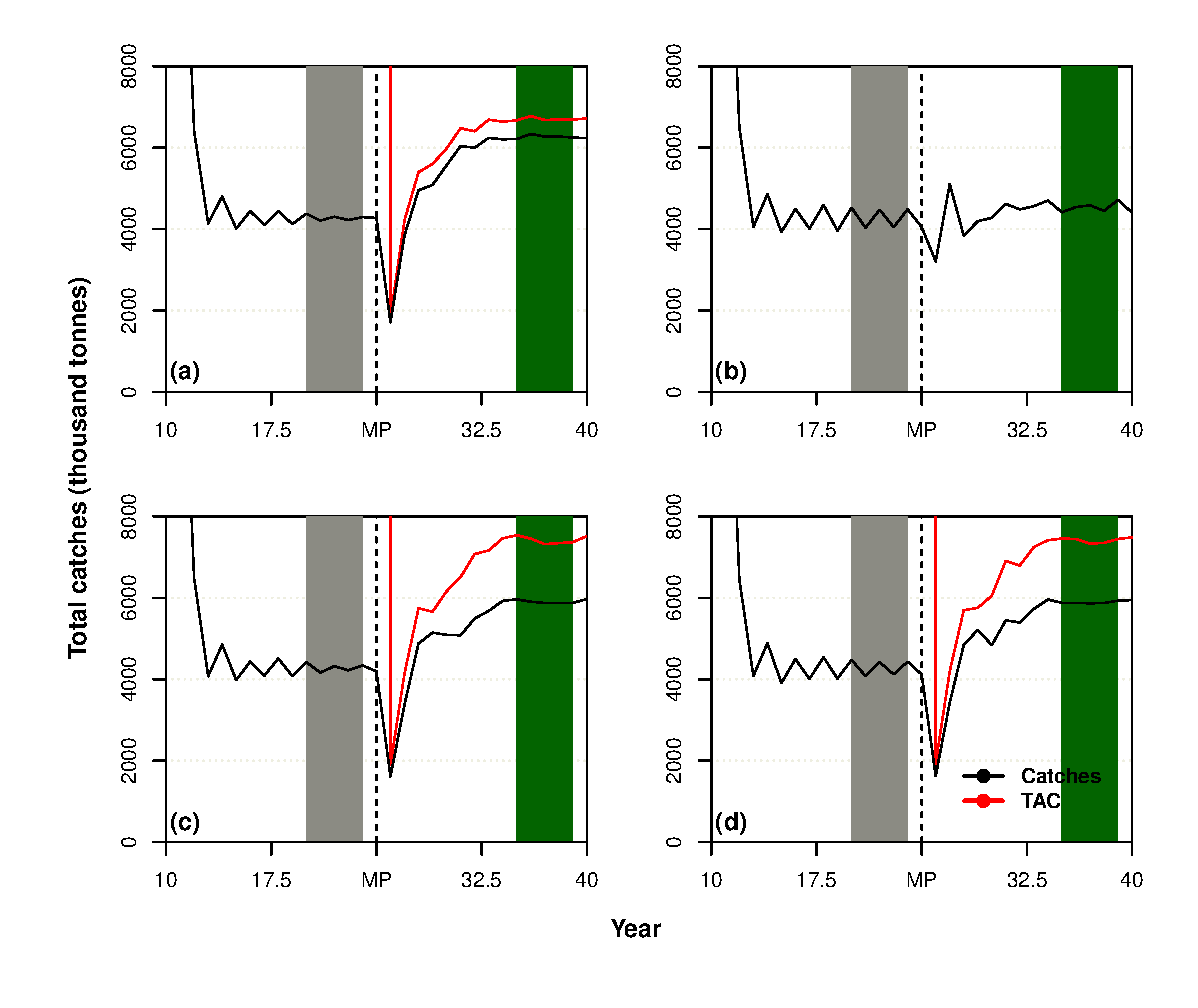
\includegraphics[width=0.8\textwidth]{Figures/Catches.eps} 
\caption{Modelled total annual catches (tonnes) for all vessels and both species: species 1 (a,c) and species 2 (b,d) in relation to the available individual quota (red line). In the top panels only species 1 quota constrained the fishery (a,b), while in the bottom panels both species quota constrained the fishery (c,d). MP year reflects the year where the management plan was introduced. Grey and green areas reflect the pre- and post-manage 5-year period, respectively.}
\label{f:catches}
\end{figure}

% HARVEST RATES
Modelling results indicated that the age composition of the harvest was different during the post-manage than it was during the pre-manage period (Fig. \ref{f:selectivity}). In the pre-manage period harvesting above the $H_{max}$ (with values around 0.03, Fig. \ref{f:catches}) caused instability in both populations. Overharvesting was caused by more significant harvesting in juvenile specimens than in adults, with a downward sloping harvest rate curves over fish age (rather than selectively targeting older fish with higher price; Fig. \ref{f:selectivity}), with average harvest rates of 0.06 (Fig. \ref{f:selectivity} and \ref{f:yields}, black lines). These harvests and levels of biomass remained stable over time due to the constant recruitment introduced into the population dynamics. On the other hand, after the MP implementation, there was a immediate decrease in harvest rates with values equal to or below $H_{max}$. After a few years, in the mid-term, 2 to 6-year old fish were harvested at the same rate during the post-manage period, while yearling fish (age class 1) was harvested at lower rates (Fig. \ref{f:selectivity} and \ref{f:yields}, grey lines).

\begin{figure}[!ht]
\centering
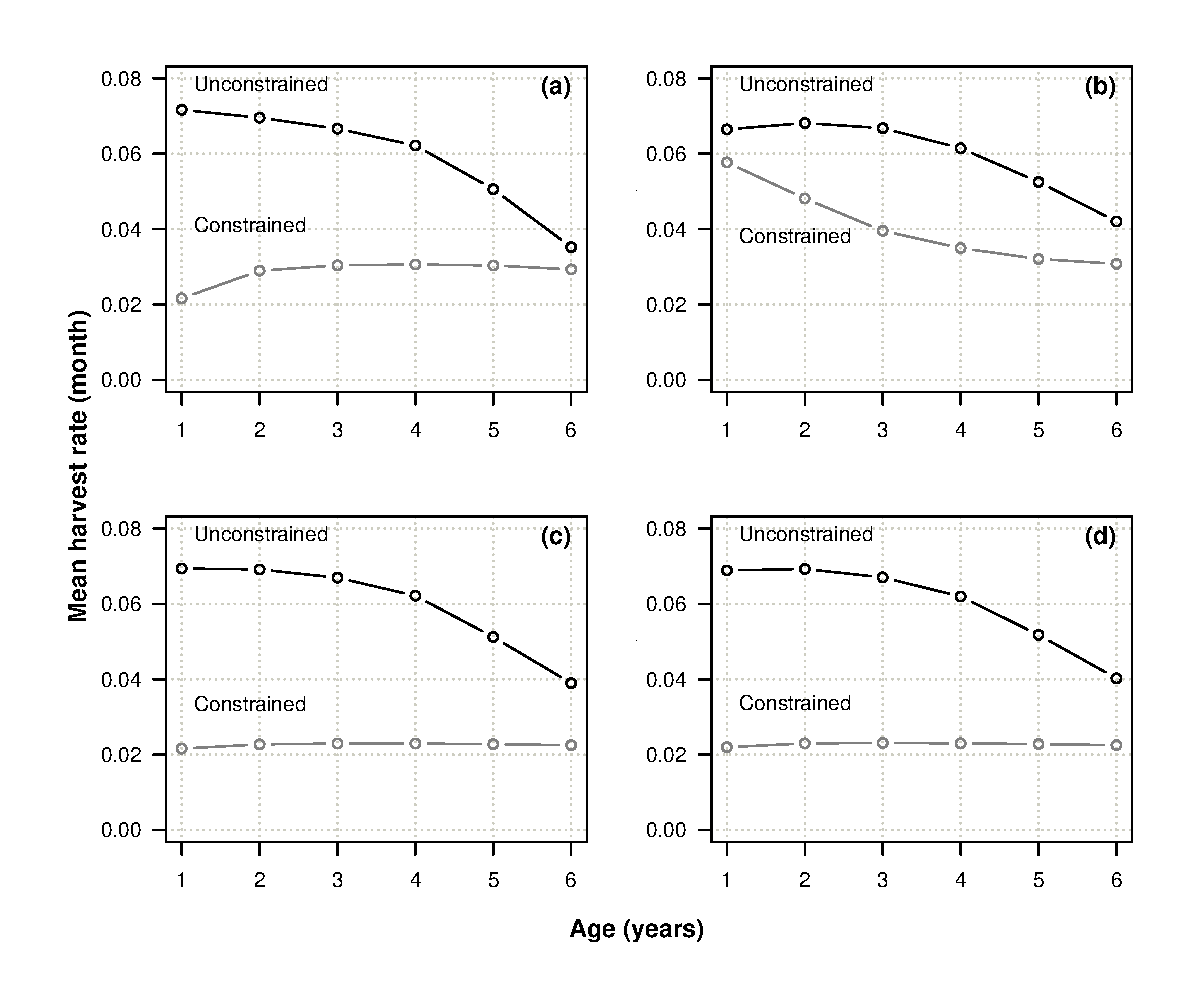
\includegraphics[width=0.8\textwidth]{Figures/Selectivity.eps} 
\caption{Modelled changes in harvest rates for both species in relation to the catch decision options made based in the available individual quota: species 1 (a,c) and species 2 (b,d). In top panels only species 1 quota constrained the fishery (a,b), while in bottom panels both species quota constrained the fishery (c,d). Black lines: mean harvest rates during the pre-manage period (unconstrained fishery); grey line: mean harvest rates during the post-manage period (constrained fishery). Periods are relative to the introduction of the management plan (grey and green areas in Fig. \ref{f:catches}).}
\label{f:selectivity}
\end{figure}
 
% YIELDS 
Expected yields as a function of harvest show that during the post-manage period both species were underharvested (Fig. \ref{f:yields}; grey lines in a,c,d), except species 2 in the single-stock quota case scenario which was overharvested due to the absence of any quota restriction (Fig. \ref{f:yields}; panel b). Indeed, higher sustainable yields achieved with lower values of fishing mortality. When quotas on both species, yields were 25\% higher than in the unmanaged situation; just on one specie quota, yield for specie 1 was 50\% higher than the unconstrained fishery value. These differences in quota scenarios could be explained due to the already commented choke effect. In general, the expected average yields shown similar values than the observed catches during the pre- and post-manage period selected; specially displaying little variability the MSY yields when accounting for quotas on both species scenario (Fig. \ref{f:yields}).

\begin{figure}[!ht]
\centering
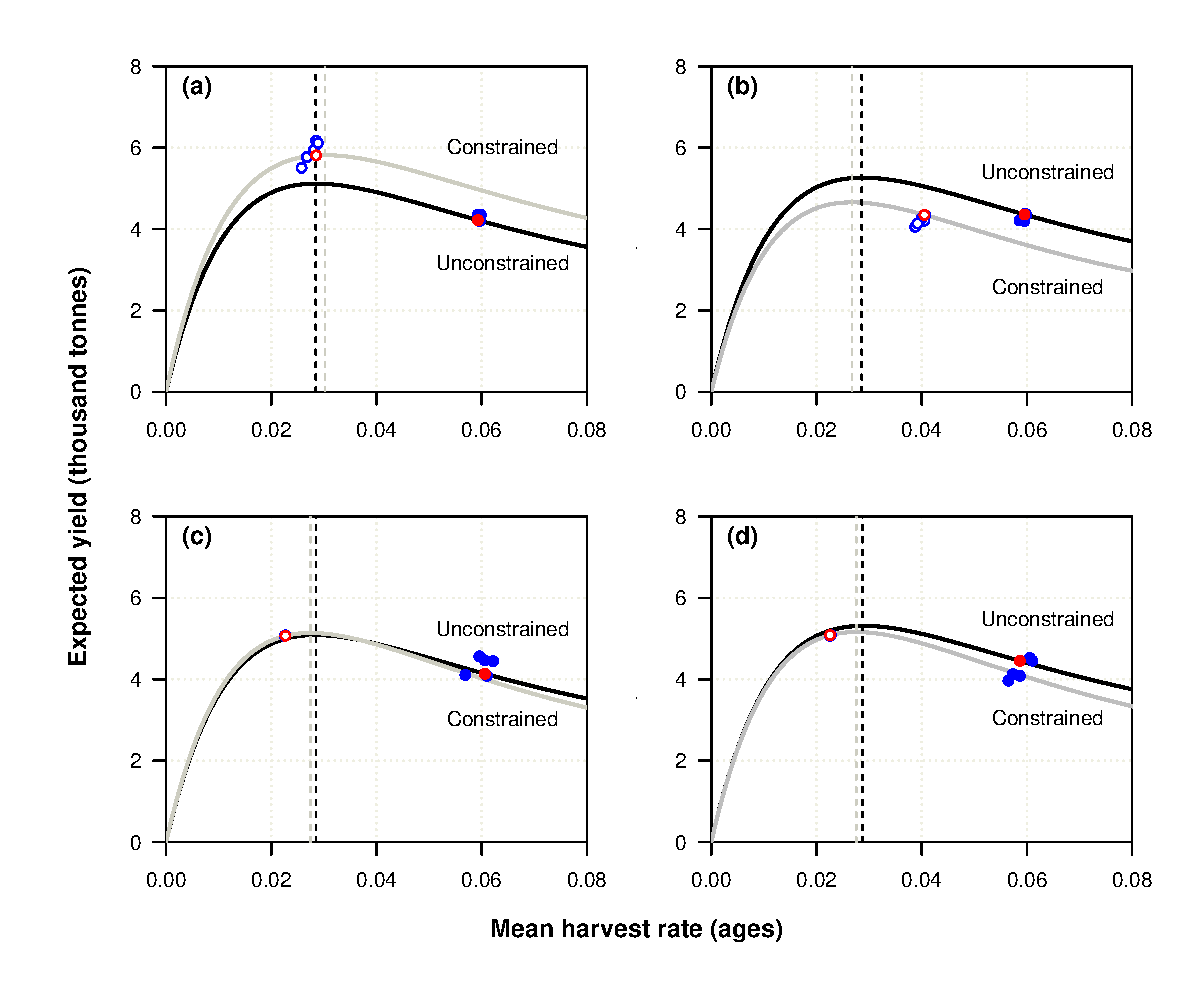
\includegraphics[width=0.8\textwidth]{Figures/Yields.eps} 
\caption{Modelled yield per recruitment curves (tonnes) for both species in relation to the introduction of the management plan: species 1 (a,c) and species 2 (b,d). In top panels only species 1 quota constrained the fishery (a,b), while in bottom panels both species quota constrained the fishery (c,d). Black lines: expected yield during the pre-manage period (unconstrained fishery); grey line: expected yield during the post-manage period (constrained fishery). Periods are relative to the introduction of the management plan (grey and green areas in Fig. \ref{f:catches}). Blue dots represent the observed catches at the mean harvest rate for each year during the 5-year period (filled dots: pre-manage period and empty dots: post-manage period), while red dots are the expected yields at sustainable harvest rates.}
\label{f:yields}
\end{figure}

% EFFORT
The fishing effort that would lead the fishery toward the biological management reference points can be seen in Figure \ref{f:effort}. In an unmanaged fishing situation, given the spatial and price distribution of the species' parameters (Fig. \ref{f:distribution} and \ref{f:prices}), fishing in both the northern and southern fishing grounds would be equally profitable. Therefore, 80\% of the fleet indistinctly choosed harvesting in both areas, with net profits of 130 thousand Euros/ year (Fig. \ref{f:effort} b and d). Fuel costs related to fishing choices were 40\% of the incurred gross revenues (Fig. \ref{f:effort} b an d). Fishing in the northern (southern) area, during the pre-manage period, showed annual average catches of 3.1 tonnes/ year and 1.2 tonnes/year of species 1 and 2, respectively (1.2 tonnes/year and 3.1 tonnes/ year), which in terms of activity would be fishing around 3100 days per area and season (Fig. \ref{f:catchesbyarea} and \ref{f:meaneffort} a and c). Some variability was appreciated between patch choices in the two scenarios (Fig. \ref{f:effort} a and c, \ref{f:catchesbyarea} and \ref{f:meaneffort}); however, gross and net revenues at the end of each year resulted in similar values (Fig\ref{f:effort} b and d). 

\begin{figure}[!ht]
\centering
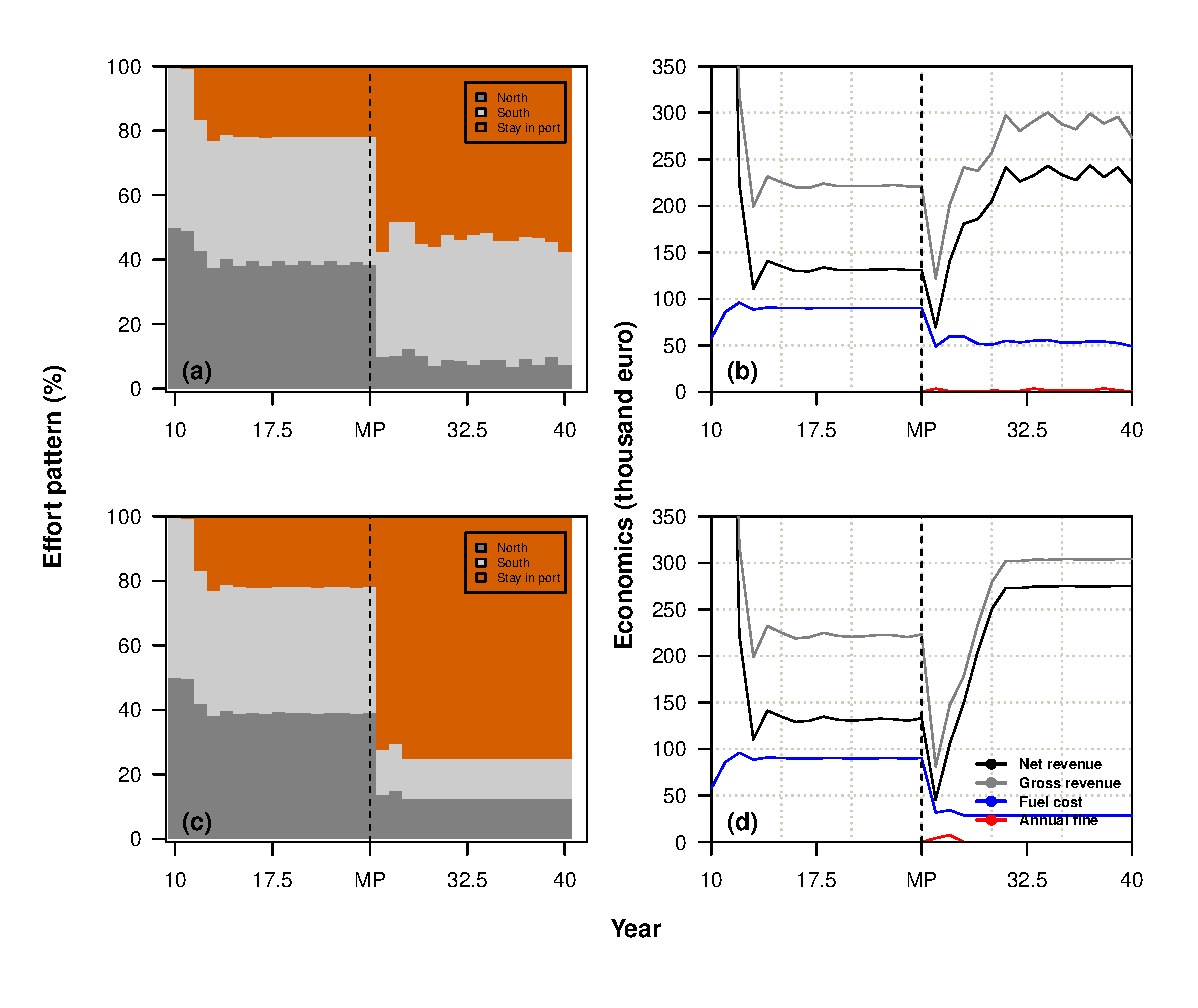
\includegraphics[width=0.8\textwidth]{Figures/Efforteconomics.eps} 
\caption{Modelled spatial allocation of effort per year (\%) and the respective economic performance when only species 1 has quota limitations (a, b) and both species are quota limited (c,d). Trade-offs between net revenue (black line), gross revenue (grey line), fuel cost (blue line) and annual fines (red line) for the fleet are shown in panels (b,d). MP years reflect the year where the management plan was introduced. In top panels only species 1 quota constrained the fishery (a,b), while in bottom panels both species quota constrained the fishery (c,d).}
\label{f:effort}
\end{figure}

When accounting in one species MSY quota, in the short-term, the fleet generated 42.31\% less revenue and a 37.50\% reduction in fishing effort than when compared to the unmanaged situation (Fig. \ref{f:effort}). At a low TAC of specie 1 in the short-term, the "effort-by-stock" required to catch species 1 TAC became smaller than the effort needed to harvest an unmanaged stock (species 2); thus, depending upon the different exploitation patterns of the fishing grounds. Therefore, vessels allocated 80\% (20\%) of the fishing effort in the southern (northern) fishing ground, while maintaining (reducing) both species catches (Fig. \ref{f:catchesbyarea}). On the other hand, such reductions in effort and changes in exploitation patterns led to an increase in stock biommass that generated a completely different picture in the mid-term. Maintaining the distribution of effort observed in the short-term, in the mid-term, the fleet would generate an average increase revenue of 76.92\% with respect to the pre-managed period, while average fuel cost were reduced to 20\% of the incurred gross revenues (Fig. \ref{f:effort} b). After the initial 57 \% to 32 \% decline in catches of species 1 and 2 due to the MP implementation, fishing in the southern (northern) area, during the post-manage period, showed in average 181.67\% and 12.87\% higher catches of species 1 and 2 than the pre-manage period, respectively (16.91\% and 38.12\% lower catches of species 1 and 2)(Fig. \ref{f:catchesbyarea} a and b). In terms of activity the average number of fishing days per season droped to 3650 days (Fig. \ref{f:meaneffort} b). Vessels were incentivized to allocate the highest amount of effort early in the year (with around 1075 and 3700 fishing days in the northern and southern fishing grounds respectively), progressively decreasing to lower levels over the course of the year (with around 121 and 1634 fishing days per area; Fig. \ref{f:meaneffort} d).

\begin{figure}[!ht]
\centering
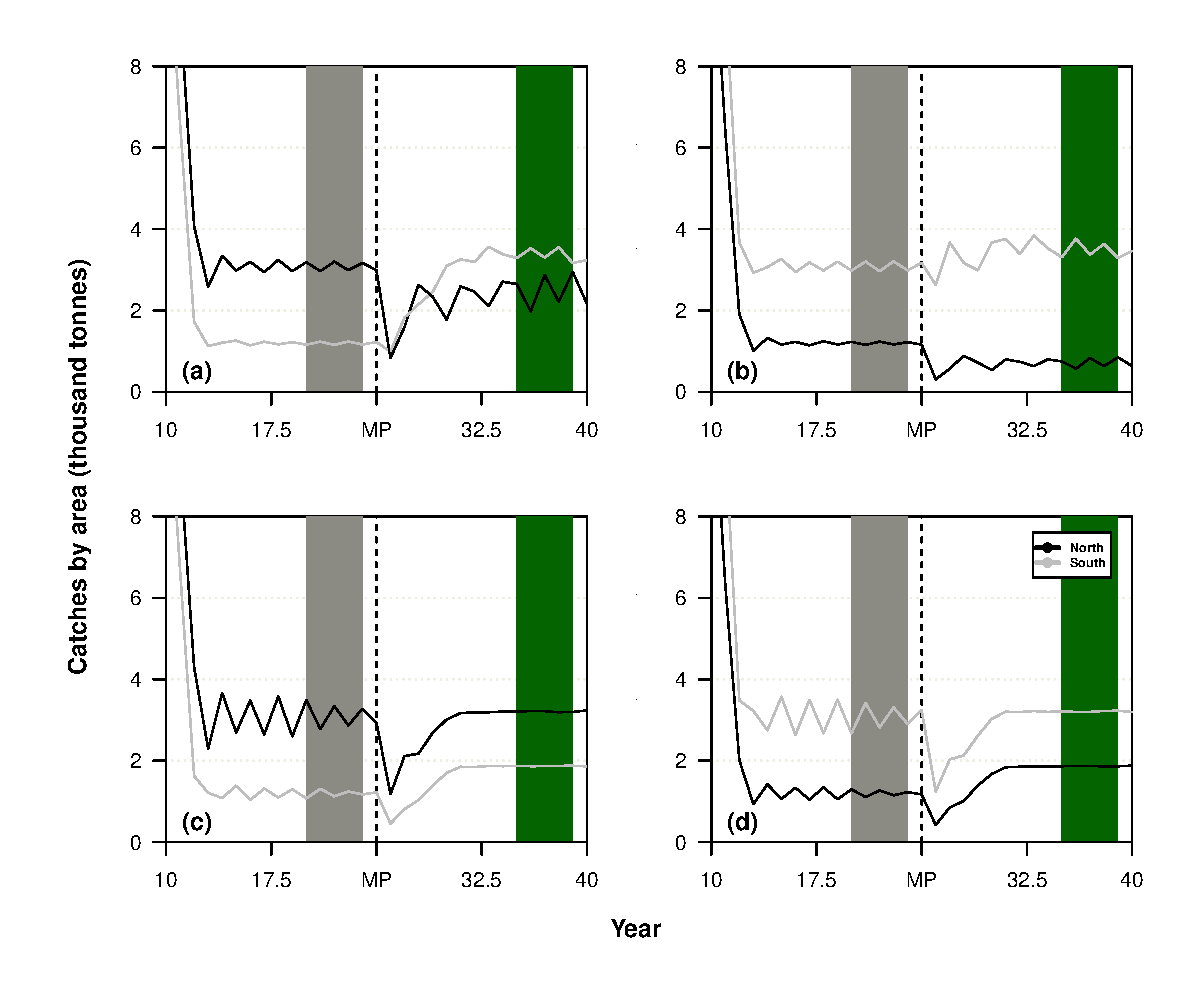
\includegraphics[width=0.8\textwidth]{Figures/Catchesbyarea.eps} 
\caption{Modelled catches (thousand tonnes/year) by area (blue line: Northern area, red line: Southern area) for both (a,c) species 1 and (b,d) species 2 in relation to the management plan period. In panels (a,b) only species 1 quota constrained the fishery, while in (c,d) both species quota constrained the fishery. MP year reflects the year where the management plan was introduced. Grey and green areas reflect the pre- and post-manage 5-year period, respectively.}
\label{f:catchesbyarea}
\end{figure} 

When accounting in MSY quotas on both species, the inclusion of one more MSY quota revealed further reductions in fishing opportunities (Fig. \ref{f:effort}). In the short-term, the fleet generated 61.54\% less revenue and a 62.5\% reduction in fishing effort than when compared to the unmanaged situation. Vessels indistinctly allocated the fishing effort in both fishing grounds (such in the pre-manage period) due to same model conditioning for both species. Therefore, after the initial 62 \% to 65 \% decline in cathes due to the MP implementation, fishing in the northern (southern) area, during the post-manage period, simulations showed in average 2.57\% and 54.54\% higher catches of species 1 and 2 than the pre-manage period, respectively (55.46\% and 4.20\%)(Fig. \ref{f:catchesbyarea} c and d). The limiting species quota incentivized vessels to choose to allocate the highest amount of effort early in the year (with around 2500 fishing days per area), progressively decreasing to lower levels over the course of the year (with around 50 fishing days per area; Fig. \ref{f:meaneffort} d). In the mid-term, the fleet would generate an average increase revenue of 107.69\% with respect to the pre-managed period. 

\begin{figure}[!ht]
\centering
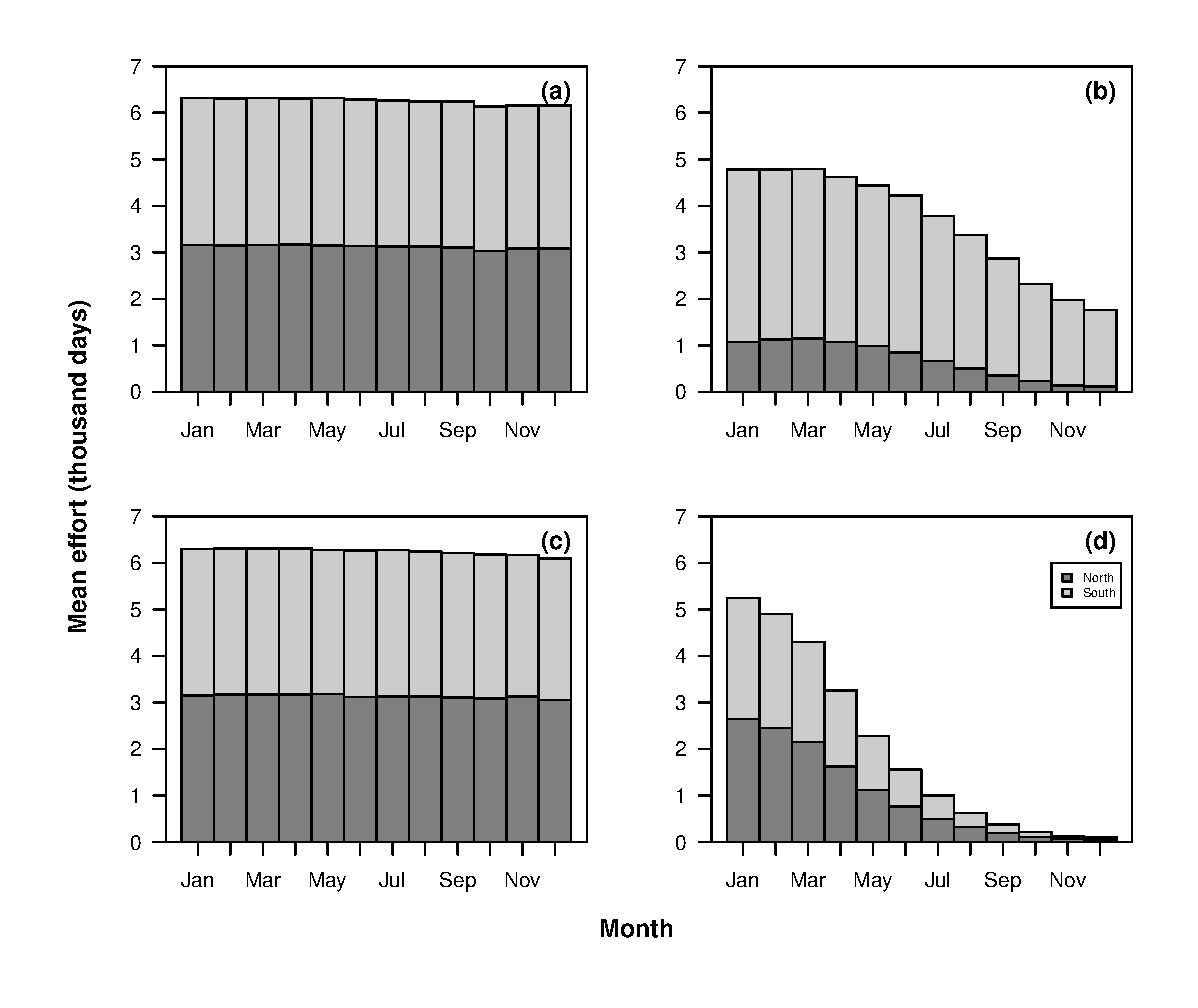
\includegraphics[width=0.8\textwidth]{Figures/Meaneffort.eps} 
\caption{Modelled average spatial allocation of effort (days/month) during the pre-manage (a,c) and post-manage periods (b,d). Periods are relative to the introduction of the management plan (grey and green areas in Fig. \ref{f:catchesbyarea}).}
\label{f:meaneffort}
\end{figure}

Modelling results suggested that moving from an unmanaged period to a sustainable stock situation, where one or both species were regulated by quotas and forced to keep fishing mortality below the MSY while it was not possible to discard, moderate and high reductions of fishing effort are expected (Fig. \ref{f:effort}, b and d). Thus, moderate to high reductions in the number of vessels modelled are expected too (effort cost per vessel 1 day; Fig. \ref{f:meaneffort}, b and d). The relative annual contribution by vessel to the gross revenue was around 28 Euros, reduced to 17 Euros of net revenues due to the costs associated to fuel during the unmanaged situation (Fig. \ref{f:meanecon}). This implies that, in the short-term, revenues under the two scenarios are predicted to result in a loss of profitability (52.89\% when accounting in one species MSY quota and 34.43\% when accounting in both MSY quota; Fig. \ref{f:meanecon}). However, in the mid-term, when compared to the pre-manage period, accounting in one species MSY quota resulted in a 1.32 times larger gross revenues per vessel; while accounting in two species MSY quotas was 1.37 times larger benefits (Fig. \ref{f:meanecon}). 

\begin{figure}[!ht]
\centering
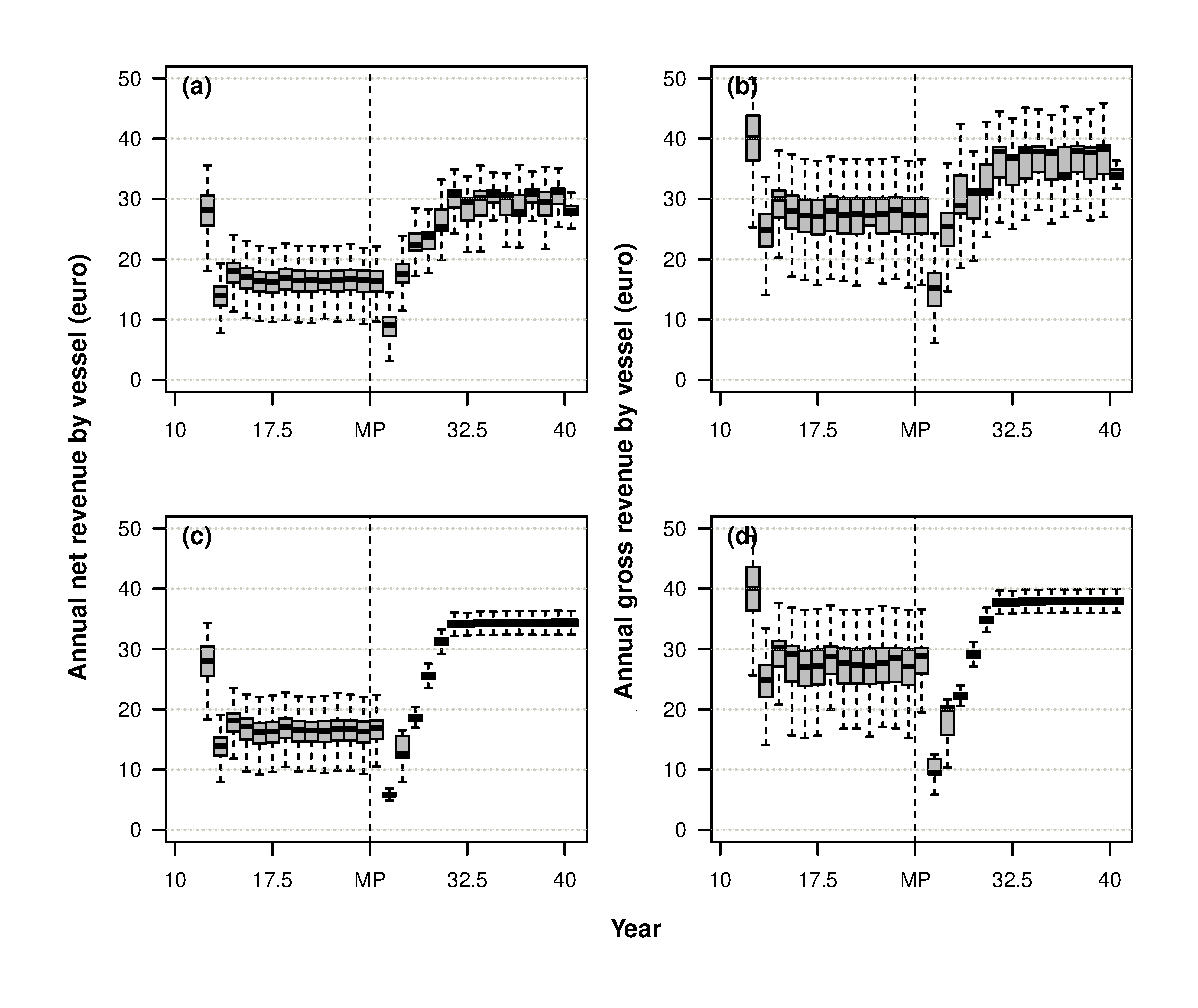
\includegraphics[width=0.8\textwidth]{Figures/Mean_Economics.eps} 
\caption{Modelled main economics by vessel (euro/ year): median annual net revenues (a,c) and median gross revenues (b,d) with the upper and lower limits of the box being the third and first quartile1 (75th and 25th percentile) respectively. MP year reflects the year where the management plan was introduced.}
\label{f:meanecon}
\end{figure}
%---

\section{Discussion}

Our results suggest that in mixed fisheries, constraining quota for a single-species can bring risk of eroding the production potential of unconstrained species. The only prerequisite for this to happen is a difference in the spatial ontogeny of the species: species differed only in the location of their nursery habitat. Growth, recruitment numbers, mortality, and price were the same for both species. Changes in quota constraints led to a spatial redistribution of the fishery and as a result of this  redistribution the age-dependent exploitation for both species changed. For the unconstrained species, the quota resulted in a shift of the fishing pressure towards younger ages. This in turn decreased the production of the unmanaged stock, as can be seen from the yield curves (Fig. \ref{f:selectivity}). 

Meanwhile, when constraining both species, the production potential of both stocks was maintained, that is to say the yield curves were unchanged. However, individual quota cobined with the stochastic fisheries catches resulted in lower than intended exploitation rates. The TACs were set so that the total TACs corresponded to the harvest rate that resulted in maximum sustainable yields. The TACs were divided in individual quotas for each fishing vessel. The lower than intended harvest rates were caused by the fact that despite their planning, fishers often exhausted one of the quotas before the other. If discarding is not allowed, then individual fishers must then stop fishing. At the population levels of the two species this resulted in overal cacthes that were lower than the TACs. Such lack of achieving MSY in mixed fisheries with multiple single-species quota has been described elsewhere \cite{Kempf2016, Rindorf2017, Hilborn2015}, but is generall attributed to differences in life-histories among fished species. In this study, the discrepancy between the intended annual quotas at MSY and realized catches is caused only by schochasticity in the system. This stochasticy in catch rates is observed in most fisheries  \cite{Sampson1988, VanOostenbrugge2004, Smith1980, Bernasconi2015}. It is caused by the complex migration biology and the effects of environmental factors on fish behaviour. A well functioning quota market would allow vessels to swap excess quota for constraining and thus bring realized catches closer to quotas. 

The model aimed to evaluate the biological and economic effects of adopting a major policy change such as the CFP \cite{CFP2013}. Starting from an overfished mixed fishery under open access conditions but with a landing obligation, the response of individual effort allocation and the interannual population dynamics are explicitly modeled, while adopting MSY objectives. The analysis extended earlier approaches that used short-term state-dependent decision-making models (e.g. \cite{Alzorriz2018, Batsleer2016, Poos2010}) by including interannual population dynamics of fish stocks, and a management procedure that mimics the decisions of a management system. Such an MSE framework was thought of as a minimum realistic model \cite{Kell2007, Punt1995}. To keep the outcomes of the model simple, and to show the implications of the fishing effort allocation, the two fish populations modelled here are exactly the same apart from their spatial distribution difference (Fig. \ref{f:distribution}). As a result, if the landing obligation changes selectivity patterns in the short-term as predicted in \cite{Alzorriz2018, Batsleer2016}, the present MSE modeling approach allows the evaluation on the reference points for sustainable exploitation in longer terms by explicitly modelling how changes in exploitation rates impact fish populations and yields. ERROR IN DECISION MAKING, NO DISCARING ALLOWED BY FISHERS, AND PERFECT COMPLIANCE TO THIS


The forecasted effects of fisheries management in mixed fisheries result from spatial heterogeneity in resources and fishers adaptive behaviour. This emphasizes that human behaviour and decision-making are intrinsic parts of conservation and natural resource management and the need for incorporating detailed fishing dynamics in management strategy evaluation. Historically, the focus of management strategy evaluation has been primarily on population dynamics in single and multispecies fisheries \cite{Butterworth2007, Dichmont2006b, Punt1999, Punt2009, Smith1999, Punt2016}. Explicitly incorporating direct effects of human behaviour of those who harvest stocks is equally important \cite{Fulton2011,Milner-Gulland2012}, but relatively few studies have attempted this \cite{Andersen2010, Ono2018}. Our MSE that links a dynamic state variable model for fisher behavior to a multi-species age structured model provides an alternative to those approaches.


When the studied mixed fishery was unmanaged, with unconstrained quota for both species (pre-manage period) and no discarding allowance, the observed harvesting rates showed average values larger than the estimated average values that can be harvested in a sustainable manner ($H_{max}$). Overfishing occurs in both stocks when fishers exceed $H_{max}$, whereas rebuilding requires reducing exploitation below $H_{max}$ (Fig. \ref{f:yields}). Therefore, during the pre-manage period, a high exploitation rate caused a decline in total biomass and fishers mainly harvest the individuals that would normally be added to the population, with younger fish being targeted for. Our results suggested that given the spatial and price species distribution parameters (Fig. \ref{f:distribution} and \ref{f:prices}), fishing in both the northern and southern fishing grounds were equally profitable; thus, the distribution of fishing effort was equally distributed (Fig. \ref{f:effort}). 

Moving from an unmanaged period to a situation where one or both species were quota regulated by implementing MSY objectives while maintaining a LO management regime (i.e. main CFP objectives: exploiting at MSY and no discarding allowance) led to a very restrictive fishing activity (Fig. \ref{f:effort}). Fishing effort was constrained by one or two quota stocks, as predicted in general terms by \cite{Ulrich2017}, resulting in drastic reductions of effort over the short-term and mid-term. In addition to reconciling fishery and conservation objectives (such as the CFP), setting exploitation rates below $H_{max}$ resulted in a reduction in fishing cost and an increase in net revenue over the mid-term (Fig. \ref{f:effort}). However, as \cite{Prellezo2016a} concluded, since effort was drastically reduced to achieve the objectives of the CFP; the increase in net revenue gains were only experienced by some vessels. Consequently, a significant part of the fleet had to cease its activity (Fig. \ref{f:effort}).

Nevertheless, the framework used made several assumptions: that there was perfect knowledge of the stochastic nature of catch rates, full compliance of fishers with the discarding policy, lack of transferability of individual quotas, and lack of interference competition among fishers \cite{Alzorriz2018}. IMPORTANT< UTILITY FUNCTION IS ANNUAL NET REV, NO SOCIAL DYNAMICS. Regarding fish populations, also important assumptions were established: negligible natural mortality, constant recruitment, constant growth, constant migration, and constant size-dependent prices. Individual choices on fishing behaviour were assumed to be made once a month. However, despite these assumptions, the minimum realistic model developed in this study allowed us to simulate the dynamics of a mixed fishery and examine the effects of single species quota management. 

In the study, the fishes were not allowed to discard, complying to a landings obligation.We did not include the use of any discard flexibilities of the LO (CFP Article 15, \cite{CFP2013}) or annaul quota swaps. Allowing the latter could potentially remedy the underutilisation of quota in the two quota situation, given that this reuslts from the stochsticity in catches, which are uncorrelated.

 We may thus have underestimated the flexibility of the fishery to respond to quota limitations imposed under both the landing obligation and exploiting at MSY. However, applying any kind of exemption or flexibility beyond the MSY would be negative \cite{Prellezo2016}. Consequently, a critical feature of management bodies is to ensure that the use of different flexibilities will constrain catches to comply with the MSY objective in Article 2(2) of the CFP Basic Regulation. Achieving a balance between quota flexibility, over-exploitation risk, and administrative simplicity is critical for the profitability and sustainability of multi-species fisheries \cite{Alzorriz2018}. The success of any new regulation also depends on achieving a balance between the costs and benefits of measures that promote voluntary compliance and those that punish non-compliance. With poor enforcement the economic benefits of non-compliance outweigh the risks of detection \cite{Batsleer2013}. In this MSE framework, detection rates were assumed to be 100\% and fines were set sufficiently high so that no discarding occurred, reflecting full compliance with regulations. However, if detection rates are low and the short-term benefits of non-compliance are high (as our results suggest) then non-compliance is likely to be a substantial problem in the absence of measures promoting voluntary compliance. IF YOU WANT TO STUDY THIS, THEN DETAILED PARAMETRIZATION IS NEEDED THAT INCLUDES CASE DEPENDENT LH CHARATRISTICS AND MIGRATIONS
 %Optimal effort at MSY generates effort reductions of 37\% to 62\% over the mid-term, thus there would be some vessels that could benefit up to 1.7 times larger profits than before the CFP implementation. The results highlighted the importance of accounting for technical interactions and their temporal dynamics in both quota allocation and fleet dynamics to design a realistic multispecies fishery management strategy analysis

Finally, a dynamic state variable model was used as a tool to create a quick quota allocation and fleet dynamics model. Many detailed fleet dynamics models have been developed over the past decades \cite{Andersen2010, Ono2018, Simons2015a} and they could have been used to include spatial factors as another dimension in the MSE. However, following \cite{Dowling2011}, incorporating uncertainty in errors in human dynamic decision-making help us to understant and predict changes in human behaviour in response of adopting a major policy change such as the CFP \cite{CFP2013}. The effect of introducing a realistic multispecies fishery within this MSE framework still remains the next step to be taken. Modelling and predicting realistic human behavior with its associated uncertainty in an ever-changing socioecological system will remain a major challenge to address in the future \cite{Ono2018}.


\section{Conclusions}

Achieving optimal yield from mixed fisheries is a pervasive problem in fisheries management (e.g., \cite{Farcas2016, Prellezo2016b, Salomon2014, Ulrich2017, Voss2014}). A multispecies fishery MSE framework based on two populations was developed in this study to examine different management scenarios. The results highlight pitfalls in managing mixed fisheries where erosion of production potential can take place, or unintentional underharvesting. We argue for the inclusion of spatial dynamics and fleet dynamics when designing a multispecies fishery management strategy evaluation. Such MSE should be done when adopting a major policy change such as the CFP. Future studies aimed at building a realistic multispecies fishery MSE with significant discard constraints, and should consider expanding the current model to include the whole suite of species exploited and managed in a real mixed fishery. The results highlighted the importance of accounting for technical interactions and their temporal dynamics in both quota allocation and fleet dynamics to design a realistic multispecies fishery management strategy analysis.

%Although this may seem implausible too, a drastic reduction of effort would increase profits if MSY and LO were contemplated. However, no flexibilities or year transfer swaps were consider. Be carefull if applying flexibilities, because as Prellezo said, any increased in mortality beyond the MSY would be negative...
%prellezo 2016, In the mid-term and without any consideration made in terms of the ecosystem functioning as a whole, the results obtained from applying any kind of exemption or flexibility are, simply, negative. Fishing beyond FMSY (even in one year) implies that there will be a penalty in the future. This penalty will come in the form of lower biomasses, that has the mixed effect of increasing the cost of fishing the same level of catches and reducing the total catch due to the lower abundances and the subsequent lower TACs.

%The largest yield (or catch) that can be taken from a species' stock over an indefinite period. Fundamental to the notion of sustainable harvest, the concept of MSY aims to maintain the population size at the point of maximum growth rate by harvesting the individuals that would normally be added to the population, allowing the population to continue to be productive indefinitely. Under the assumption of logistic growth, resource limitation does not constrain individuals’ reproductive rates when populations are small, but because there are few individuals, the overall yield is small. At intermediate population densities, also represented by half the carrying capacity, individuals are able to breed to their maximum rate. At this point, called the maximum sustainable yield, there is a surplus of individuals that can be harvested because growth of the population is at its maximum point due to the large number of reproducing individuals. Above this point, density dependent factors increasingly limit breeding until the population reaches carrying capacity. At this point, there are no surplus individuals to be harvested and yield drops to zero. The maximum sustainable yield is usually higher than the optimum sustainable yield and maximum economic yield

%There is an extensive literature on fisheries economic theory in which the Gordon-Schaefer equilibrium production model is central (Gordon 1954, Schaefer 1957, Clark 1983). This theory holds that there is an economic TRP, the Maximum Economic Yield (MEY), which occurs at the effort level yielding the greatest margin of revenue over cost from the resource. 
%For a linear cost curve, this inevitably occurs to the left of MSY on the fishing effort axis. Since Fmey occurs at lower levels of effort than Fmsy, the use of this economic Target Reference Point is less likely to result in biological overfishing than the use of Fmsy.

%As a TRP, Fmey is responsive to any changes in the economic environment which affect either the value of fish, or the cost of fishing. It may also be dependent on changes in fish abundance, if market price increases with declining abundance and is independent of the availability of similar resources elsewhere. Subsidies or external economic considerations such as fuel taxes will also affect the location of an economic Reference Point (e.g. Panayotou 1988).

%The effect of supply on fish prices may, under certain circumstances, result in higher total profit, or profit per unit catch, when total catch is reduced. This characteristic may be a consideration in setting target fishing levels or catches but is least likely to be effective in situations where fish prices are set by global markets, e.g. the tuna fishery for the canning industry.

%The value of a unit weight of the landed catch may vary with the size of individual fish, and in multispecies fisheries with species composition. Both fish size and species composition are functions of fishing mortality, and based on purely economic criteria, may be used as target reference points. Even if the actual target F cannot be estimated, in theory, F could be adjusted in increments until the desirable target catch characteristics are achieved.

%In considering TRPs based on economic criteria, it is important to be aware of the effect which the practice of discounting could have on reference points. In evaluating investment projects, including resource management, economists discount the future value of any commodity. Discount rates may be in the order of 10\%. In the case of a fishery where the population growth rate does not exceed the discount rate, then a strict application of economic theory would suggest that in the absence of other considerations (such as an economic value placed on recreational use of resources) the whole stock should be harvested now, and the proceeds of their sale invested. Long-lived species with slow growth rates, such as whales, clearly fall into this category. The blatant contradiction between this common economic approach, and the concept of sustainability, constitutes an unresolved paradox (Hilborn and Walters 1992).


\begin{notes}[Acknowledgements]
The content of this paper does not reflect the official opinion of the European Commission. Responsibility for the information and views expressed in this paper relies entirely with the authors.
\end{notes}

\bibliographystyle{plain}
\bibliography{mylib}

\end{document}
